\chapter[New Loss Functions]{New Loss Functions: Comparing Asymmetric and Symmetric losses in Evaluating Error} \label{ch3:loss}
\chaptermark{New Loss Functions}
\setlength{\epigraphwidth}{4.5in}
\epigraph{Maybe all one can do is hope to end up with the right regrets.}{Arthur Miller, \textit{``The Ride Down Mount Morgan''}, 1991}

%----------------------------------------------------------------------------------------------------------------------------------------------------------------------------------------------------------
\section*{Summary}
In statistical learning, the loss function is the translation of an informal philosophical modeling objective into the formal language of mathematics \cite{hennig2007some}. Some measures-of-fit have already been established and are common in hydrologic modeling (e.g., Mean Squared Error (MSE), Nash-Sutcliffe Efficiency (NSE)). However, these loss functions are all symmetric, and the MSE is the loss function of choice in most modeling efforts. Symmetric functions produce the same loss when underpredicting and overpredicting of the same absolute error. However, an asymmetric loss function applies a different penalty to the different directions of loss. This feature allows an asymmetric loss function to force the model to overpredict unimpaired flows in times of floods and underpredict them in droughts rather than the less desirable opposite. The idea here is to make more conservative decisions, since being prepared for more extreme floods and droughts implies more conservative decisions. 

This chapter uses six loss functions: four symmetric consisting of Mean Squared Error (MSE), Log Hyperbolic Cosine (LOGCOSH), Mean Absolute Error (MAE), Mean Squared Percentage Error (MSPE), and two asymmetric consisting of Mean Weighted Least Squares Error (WLSE) and Linear Exponential Error (LINEX). It presents the results obtained by a NN model. A visual comparison of the model fits shows that the asymmetric functions, with appropriate nuisance parameter estimates, can force better fits at the peaks and valleys of a hydrograph.  

%----------------------------------------------------------------------------------------------------------------------------------------------------------------------------------------------------------
\section{Introduction}
%---------------------------------------------------
\subsection{Loss Functions in Statistical Learning}
Typical loss functions in statistical learning are the $\ell_1$-norm and $\ell_2$-norm (Equations \ref{eq:l1} and \ref{eq:l2}). The $\ell_2$-norm is the familiar objective function in simple least-squares regression, a convex function, emphasizing points distant from the bulk of the data. % (i.e., data points that have high leverage and can influence the model more than other points).

\begin{equation} \label{eq:l1}
	\ell_1(y_i,\hat{f}(x_i)) = ||y_i-\hat{f}(x_i)||_1 = \abs{y_i-\hat{f}(x_i)} 
\end{equation}
	
\begin{equation} \label{eq:l2}
	\ell_2(y_i,\hat{f}(x_i)) = ||y_i-\hat{f}(x_i)||_2^2 = \left(y_i-\hat{f}(x_i)\right)^2 
\end{equation}
 
\textit{Risk}, or cost, is defined as the expectation of the loss function. For example, the risk of overpredicting the severity of a drought can be defined as \textit{how much} it was overpredicted on average. This distance can be defined as the absolute value of the difference or the difference squared as in Equations \ref{eq:l1risk} and \ref{eq:l2risk}, the empirical risks associated with the $\ell_1$-norm and $\ell_2$-norm. The expectation of the $\ell_2$-norm will produce a model that regresses to the mean, and the $\ell_1$-norm regresses to the median. That is, the $\ell_2$-norm is more sensitive to outliers than the $\ell_1$-norm. Using either norm implies that the modeler is more concerned with a conservative measure of centrality rather than getting predictions closer to the extremes of the distribution. Asymmetric loss functions discussed later can address this issue. 

\begin{equation} \label{eq:l1risk}
	\begin{aligned}
		& L_1(y_i,\hat{f}(x_i)) = E\left[\ell_1(y_i, \hat{f}(x_i))\right] = \frac{1}{n} \sum_{i=1}^{n} \abs{y_i-\hat{f}(x_i)}
		% E\left[\abs{y_i-\hat{f}(x_i)}\right] \\
		% & L\left(\abs{y-\hat{f}(x)}\right) = \frac{1}{n} \sum_{i=1}^{n} \abs{y_i-\hat{f}(x_i)}
	\end{aligned}
\end{equation}
	
\begin{equation} \label{eq:l2risk}
	\begin{aligned}
		& L_2(y_i,\hat{f}(x_i)) = E\left[\ell_2(y_i, \hat{f}(x_i))\right] = \frac{1}{n} \sum_{i=1}^{n} {(y_i-\hat{f}(x_i))^2}
		% E\left[(y_i-\hat{f}(x_i))^2\right] \\
		% & L\left((y-\hat{f}(x))^2\right) = \frac{1}{n} \sum_{i=1}^{n} {(y_i-\hat{f}(x_i))^2}
	\end{aligned}
\end{equation}

As an aside, \textit{Regret} is the difference between the consequences of a sub optimal decision and the optimal decision. Often, in reinforcement learning, the objective is to minimize total regret, which is equivalent to maximizing the highest accumulated reward \cite{sutton2018reinforcement}. For example, maybe overpredicting the severity of a drought this year will lead to better management of resources and fewer regrets in later years. To avoid developing a mathematical representation for regret, we will proceed with the much simpler \textit{risk-minimization framework} (Equation \ref{eq:mlriskmin}). 

\begin{equation} \label{eq:mlriskmin}
	\hat{f}(x_i) = \underset{\tilde{f}}{\mathrm{argmin}} \ E\left[L(y, \tilde{f}(x))\right] \\
\end{equation}

%---------------------------------------------------
\subsection{Loss Functions in Hydrologic Modeling}
In practice, the loss function for a chosen statistical learning method is the translation of a informal philosophical modeling objective into the formal language of mathematics \cite{hennig2007some}. So, the choice of a loss function in estimation is somewhat subjective and depends on the specific application of the model or the decisions being made when used. 

Mechanistic models in hydrology simulate conditions based on available input parameters, modeled processes, and calibration to specific locations. \textit{Measures-of-fit} or the similarity of the simulations to the observations help in assessing model performance. Visual similarity is recommended as the most fundamental approach to assessing model performance (i.e., the plot of observed and simulated time series), and calculated measures-of-fit are recommended next as an objective assessment \cite{krause2005comparison}. In addition to model performance estimation, these measures can help guide better fits of simulations to observations in model calibration or ``nuisance'' parameter estimation. 

Some measures-of-fit have already been established and are common in hydrologic modeling: the Mean Absolute Error (MAE), Mean Squared Error (MSE), Root Mean Square Error (RMSE), normalized RMSE (nRMSE), RMSE standard deviation ratio (RSR), Relative Standard Deviation (RSD), Relative Mean (RMU), Percent Bias (PBIAS), Coefficient of Determination (R$^2$), Nash-Sutcliffe Efficiency (NSE), Index of Agreement (d), Modified NSE, Modified d, Relative NSE, Relative d, King-Gupta Efficiency (KGE), and Volumetric Efficiency (VE). Appendix \ref{d:mof} presents their equations, strengths, and weaknesses. 

The following is a discussion on the characteristics of the loss function in its application to hydrologic prediction:

(1) \textbf{Symmetric} vs. \textbf{Asymmetric}: In symmetric functions, underpredicting produces the same loss as overpredicting of the same absolute error. However, a conservative loss function applies a different penalty to the different directions of loss (overpredicting vs. underpredicting). So, an asymmetric loss function can force the model to over predict the unimpaired flows in times of floods and under predict them in droughts rather than the less desirable opposite. This approach requires the labeling of all instances of the data as either a peak (flood), or valley (drought) point. Therefore, we need a labeling mechanism (i.e., a classification model) before fitting the predictive regression model. 

Great care should be taken not to introduce ``data leakage'' or the inclusion of information from the response variable into the training of the predictive model; the classification model will have to either be trained on the predictor variables only, or use a portion of the data that is set aside for the rest of the study. 

Once all observations are classified, we define different loss functions for each peak and valley section. Such loss functions can be defined as linear exponential (LINEX) loss if smoothness is desired (Equation \ref{eq:linex} and Figure \ref{fig:asymmetric1}). However, current subgradient-based and derivative-free methods of optimization in convex programming can easily handle non-differentiability at the origin of the loss function. Many asymmetric loss functions in machine learning have a simple \textit{kink} in them. They are otherwise entirely differentiable (Equation \ref{eq:asshinge} and Figure \ref{fig:asymmetric3}).

\begin{figure}[ht]
	\centering
	\begin{subfigure}{.49\textwidth}
  		\centering
 		 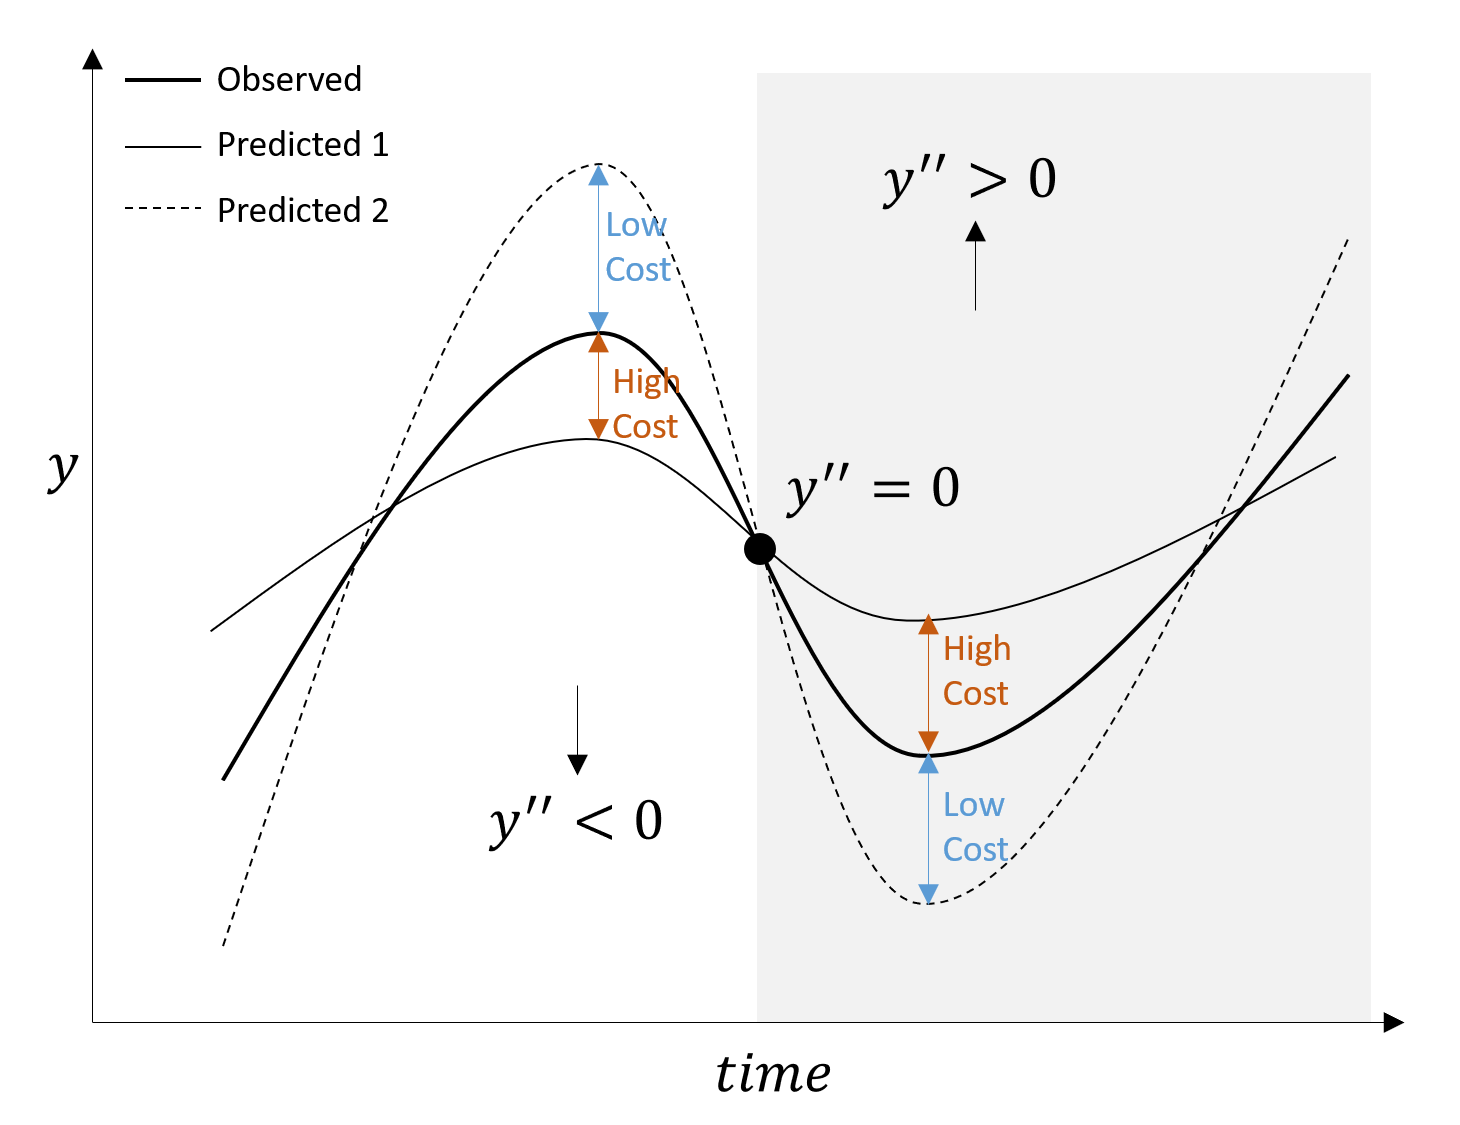
\includegraphics[width=\textwidth, trim={0 0 0 0}, clip=true]{plots/ch3_asymmetric1_a.png}
  		\caption{Desired asymmetricity in peaks and valleys}
  		\label{fig:asymmetric1a}
	\end{subfigure}% 
	\begin{subfigure}{.49\textwidth}
  		\centering
  		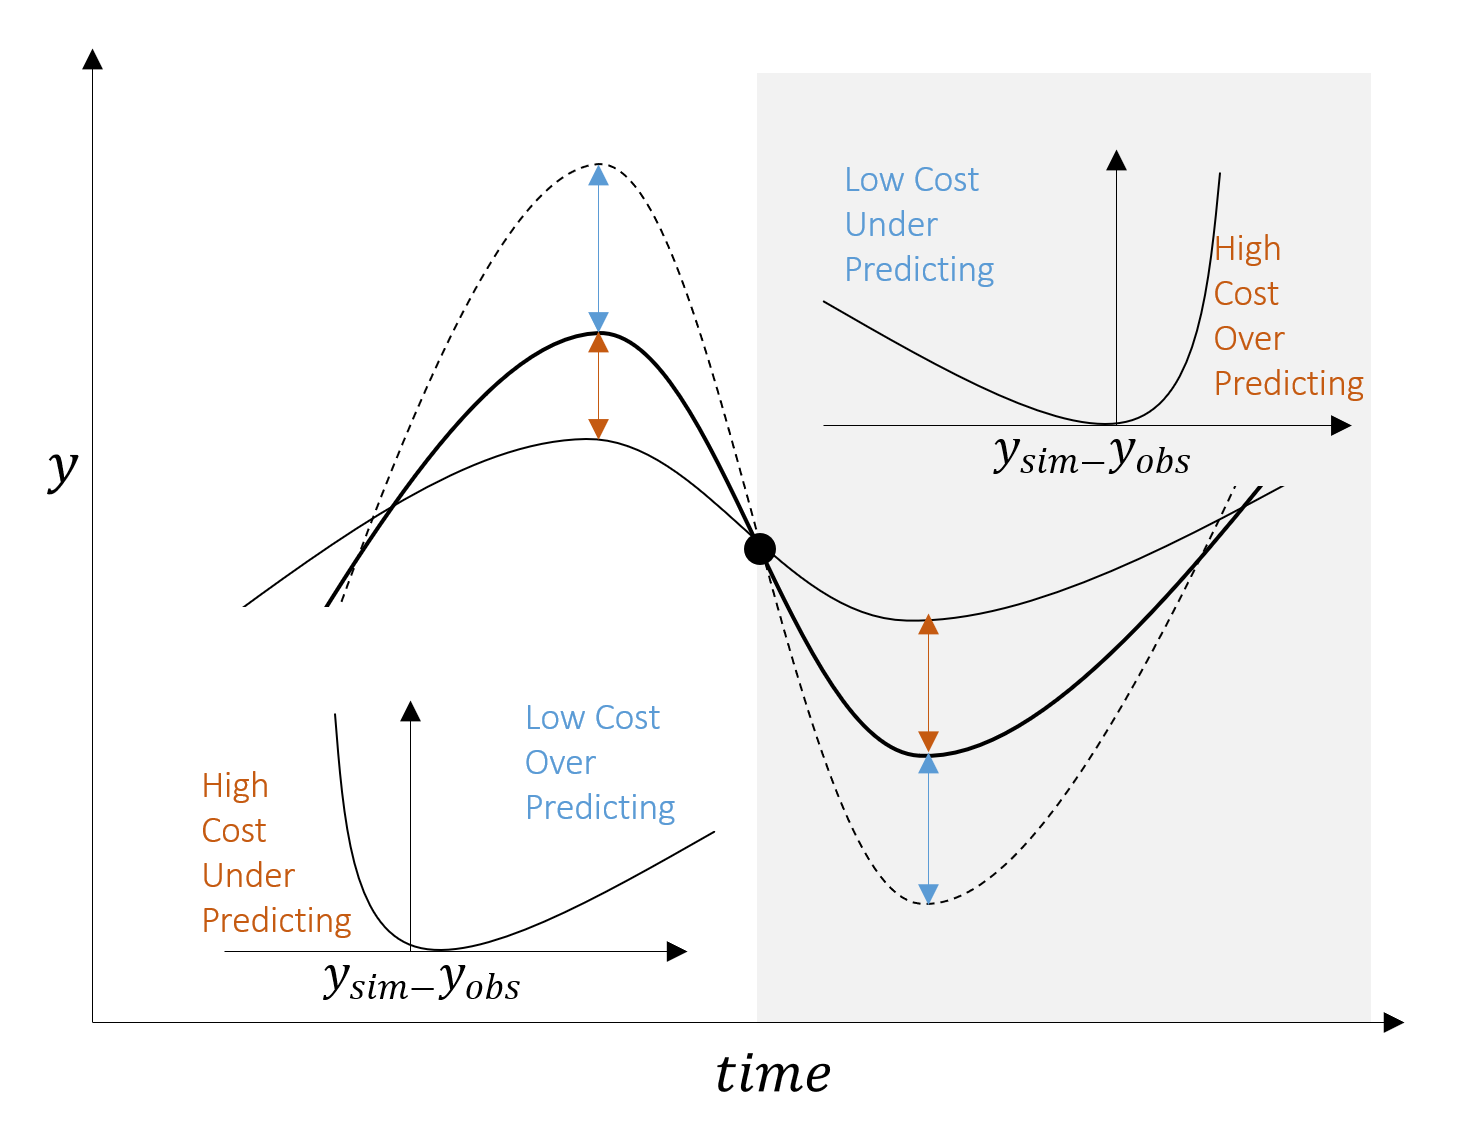
\includegraphics[width=\textwidth, trim={0 0 0 0}, clip=true]{plots/ch3_asymmetric1_b.png}
  		\caption{Asymmetric loss defined with LINEX}
  		\label{fig:asymmetric1b}
	\end{subfigure}
	\caption[Asymmetric loss functions.]{Asymmetric loss functions define different losses to overpredicting and underpredicting a value. A positive $\protect\phi$ defines the LINEXE needed for drought cases and a negative $\protect\phi$ for flood cases.}
	\label{fig:asymmetric1}
\end{figure}

\begin{equation} \label{eq:linex}
	LINEX(y_i,\hat{f}(x_i)) = e^{\phi(y_i-\hat{f}(x_i))} - \phi(y_i-\hat{f}(x_i))-1, \quad\text{$\phi$} \in \mathbb{R}
\end{equation}

\begin{figure}[ht]
	\centering
	\begin{subfigure}{.49\textwidth}
  		\centering
 		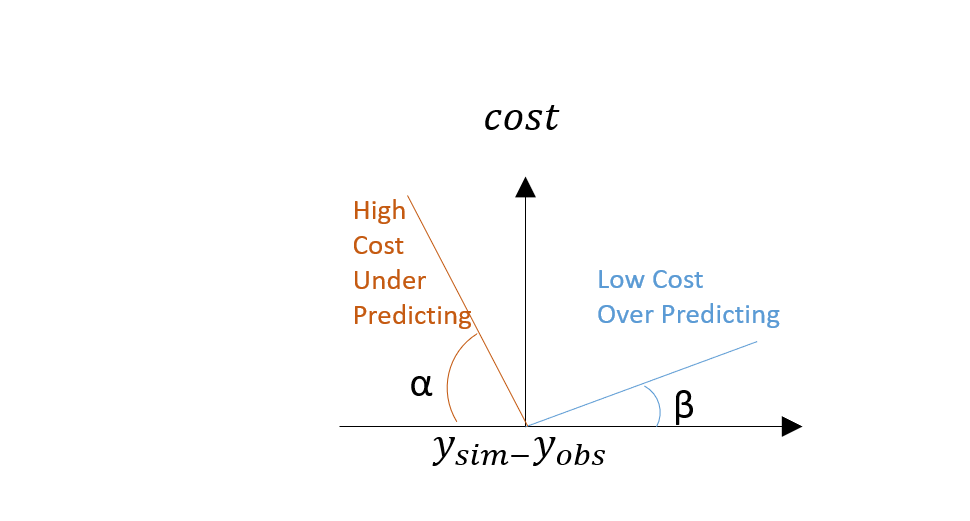
\includegraphics[width=\textwidth, trim={0 0 0 0}, clip=true]{plots/ch3_asymmetric3_a.png}
  		\caption{Floods}
  		\label{fig:asymmetric3a}
	\end{subfigure}% 
	\begin{subfigure}{.49\textwidth}
  		\centering
  		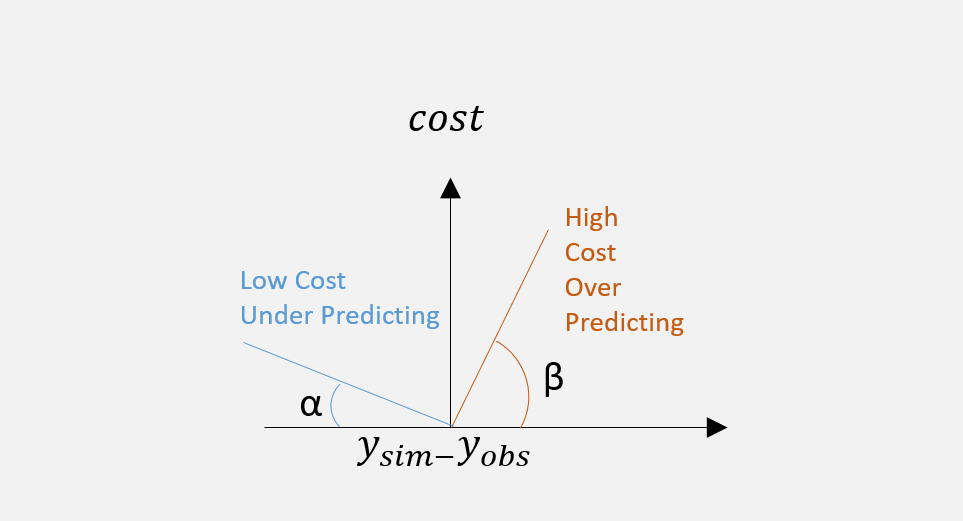
\includegraphics[width=\textwidth, trim={0 0 0 0}, clip=true]{plots/ch3_asymmetric3_b.png}
  		\caption{Droughts}
  		\label{fig:asymmetric3b}
	\end{subfigure}
	\caption[Asymmetric weighted absolute value loss function.]{An asymmetric weighted absolute value loss function can define different slopes to overpredicting and underpredicting a value.}
	\label{fig:asymmetric3}
\end{figure}

\begin{equation} \label{eq:asshinge}
	Hinge(y_i,\hat{f}(x_i)) = \alpha*min(0, \hat{f}(x_i)-y_i)+ \beta*max(0, \hat{f}(x_i)-y_i)
\end{equation}

The squared error loss penalizes larger errors more than smaller error; the function is steeper in the tails than in the middle. To preserve this feature, we can combine the concepts above and define a weighted $\ell_2$-norm (Equation \ref{eq:weightedse}). 

\begin{multline} \label{eq:weightedse}
	Weighted\ Squared\ Error(y_i,\hat{f}(x_i)) = \alpha*\left[min\left(0, (\hat{f}(x_i)-y_i)\right)\right]^2 \\
	+ \beta*\left[max\left(0, (\hat{f}(x_i)-y_i)\right)\right]^2
\end{multline}

% define and explain LOGCOSH!!!!!!!!!

% I put this in appendix B, terms
%Figure \ref{fig:curves} shows the functions discussed above. 
%
%\begin{figure}[ht]
%	\centering
% 	\includegraphics[width=\textwidth, trim={0 0 0 0}, clip=true]{plots/rplot31_lossfuncs3.png}
%	\caption{Typical loss functions.}
%	\label{fig:curves}
%\end{figure}

(2) \textbf{Relative Errors} vs. \textbf{Absolute Errors}: In hydrology, manual and automatic attempts aimed at minimizing absolute errors often lead to fitting the higher portions of the hydrograph (peak flows) at the expense of the lower portions (baseflow) \cite{krause2005comparison}. Relative errors are generally more important than absolute errors unless the goal is to estimate water supply. For example, depending on the modeling purpose, a 100 TAF error in 1,800 TAF (monthly annual average of the Sacramento River) could be a less extreme error than in 300 TAF (monthly annual average of the Trinity River). Relative error loss functions or a simple log transformation of the data can help in this regard. We have used one relative error loss function, the Mean Squared Percentage Error (MSPE), for illustrative purposes. 

(3) \textbf{Continuous} vs. \textbf{Step-wise}: Although, most outcomes may follow a discontinuous step function (e.g., a neuron firing or not), many decisions in water resources (e.g., releases from a reservoir) are continuous. Continuity and differentiability make continuous math more convenient. One major development in neural networks was doing away with the concept of thresholds in the step function (representing the collective influence of all the inputs) and replacing it with a smoother \textit{sigmoid} function. As with neural networks, many optimization algorithms require continuity and differentiability (e.g., gradient decent). However, advances in these methods now allow for piece-wise differentiability in the loss function. To make matters simple, we use continuous functions. 

(4) \textbf{Homogeneous} vs. \textbf{Heterogeneous (i.e., weighted based on geographic region)}: The cost of incorrectly managing a densely populated urban basin may be very different than a desert or a headwater basin; the importance of having accurate flow estimates is not completely homogeneous especially across a big and diverse region like California. However, to avoid making those judgments, we use a single loss function across all regions. 
% could use cost functions that differentiate between the costs of predicting the wrong hydrology for a populated basin and the same costs for fish species. % should costs from CALVIN? cost of not delivering the target demand. is that the same cost as not predicting the hydrology right? not really. 

% \citeA{legates1999evaluating} suggests that a complete assessment of model performance should include at least one \textit{goodness-of-fit} or relative error measure (e.g., Mean Absolute Logarithmic Error defined in ????) and at least one absolute error measure (e.g., MSE or MAE defined in Equation \ref{eq:mse} \& \ref{eq:mae}) with additional supporting information (e.g., a comparison between the observed and simulated mean and standard deviations such as those defined in Equation \ref{eq:rsd} \& \ref{eq:rmu}) \cite{legates1999evaluating}. 

%-----------------------------------------------------------------------------------------------------------------------------------------------------------------------------------------------------
\section{Methods}
Table \ref{table:lossfuncs} shows the loss functions used in the NN model. 

\begin{table*}[h]\renewcommand{\arraystretch}{0.8} 
	\linespread{0.5}
	\centering
	\caption{Loss functions used in NN model.}
	\begin{tabular}{p{1.2cm}p{2.4cm}p{4.7cm}p{6.5cm}} % must add to 14.8
		\toprule
		Type$^{\ast}$ & Abb. & Name & Function\\
		\midrule
		S & MSE & Mean Squared Error & keras::loss\_mean\_squared\_error()\\
		\addlinespace
		S & LOGCOSH & Log Hyperbolic Cosine & keras::loss\_logcosh()\\
		\addlinespace
		S & MAE & Mean Absolute Error & keras::loss\_mean\_absolute\_error()\\
		\addlinespace
		S & MSPE & Mean Squared Percentage Error & custom\_metric (code below)\\
		\addlinespace
		A & WLSE & Mean Weighted Least Squares Error & custom\_metric (code below)\\
		\addlinespace
		A & LINEXE & Linear Exponential Error & custom\_metric (code below)\\
		\bottomrule
	\end{tabular}
   	\begin{tablenotes}
      		\small
      		\item $^{\ast}$ S: Symmetric; A: Asymmetric
	\end{tablenotes}
	\label{table:lossfuncs}
\end{table*}

% This can be defined by a fit of a thin plate spline to the precipitation data with a predefined degree of smoothness (i.e., degree of freedom). Next, we find the points at which the direction of curvature (the second derivative) in the time series changes. Areas where the curvature is upward can be labelled drought and downward labelled flood. 
In asymmetric loss functions, a simple classification model is needed to label points as flood (``FLOOD''==1) and drought (``FLOOD''==0). For each basin, the mean precipitation across the full record was designated a hard threshold; if the precipitation of a given month fell below this value, that observation was designated a ``drought'' and if above, a ``flood''. Given this designation, we can apply different losses to the prediction error at different locations in the hydrograph. 

Another consideration had to be made for defining loss functions in {\tt keras}. Losses in {\tt keras} can accept only two arguments: y\_true and y\_pred, which are the target tensor and model output tensor, respectively. However, if we desire the loss to depend on other tensors-as is the case with asymmetric losses-we are required to use ``function closures.'' Here, the loss function takes in whatever arguments we desire and returns the function that only depends on y\_true and y\_pred. Hence, the name ``wrappers.'' Code snippets for the WLSE and LINEXE wrappers show how this is accomplished. 

Also, since we now have labeled observations (floods or droughts), we need this designation to line up with each y\_true and y\_pred correctly. Therefore, we can no longer use ``minibatch'' training methods that scramble the data without significantly changing the scrambling algorithm to accommodate labels. The size of the minibatch is determined by the validation split (e.g, 0.2) and only aids in speeding up the model training. To still make accurate predictions without minibatch, we simply increased the training epochs from 100 to 1000.  Note that in this case, shuffle=FALSE. 

The following snippets of R code show how the custom losses were defined. 

MSPE loss is defined as follows:
\begin{lstlisting}[literate={<-}{{$\gets$}}1]
	mspe <- function(y_true, y_pred){
	  K <- backend()
	  # added a 1 to y_true in the denominator, because dividing by 0 is a problem. You can also use a relu function, or use a clip where the 0 values get truncated. However, here, in the cases where y_true=0, the mspe function turns into a simple mse.
	  mod_loss <- K$mean(K$pow((K$flatten(y_pred)-K$flatten(y_true))/K$flatten(y_true+1), 2))
	  return(mod_loss)
	}
\end{lstlisting}

WLSE loss is defined as follows: 
\begin{lstlisting}[literate={<-}{{$\gets$}}1]
	wlse <- function(y_true, y_pred, flood_vect, alphad, betad, alphaf, betaf){
	  alpha_vect <- ifelse(flood_vect==0, alphad, alphaf)
	  beta_vect <- ifelse(flood_vect==0, betad, betaf)
	  K <- backend()
	  alpha_vect_cte <- K$constant(alpha_vect, dtype='float32')
	  beta_vect_cte <- K$constant(beta_vect, dtype='float32')
	  alpha_loss <- K$transpose(alpha_vect_cte)*K$cast(K$pow(K$minimum(0, K$flatten(y_pred)-K$flatten(y_true)), 2), dtype='float32')
	  beta_loss <- K$transpose(beta_vect_cte)*K$cast(K$pow(K$maximum(0, K$flatten(y_pred)-K$flatten(y_true)), 2), dtype='float32')
	  mod_loss <- K$sum(alpha_loss + beta_loss)*10^-6
	  return(mod_loss)
	}
\end{lstlisting}

WLSE wrapper is defined as follows: 
\begin{lstlisting}[literate={<-}{{$\gets$}}1]
	wlse_wrapper_stochastic <- custom_metric("wlse", function(y_true, y_pred) {wlse(y_true, y_pred, flood_vect=trainsetpvs[, "FLOOD"], alphad=0.00001, betad=0.00005, alphaf=0.00005, betaf=0.00001)})
\end{lstlisting}

LINEXE loss is defined as follows:
\begin{lstlisting}[literate={<-}{{$\gets$}}1]
	linexe <- function(y_true, y_pred, flood_vect, phid, phif){
	  phi_vect <- ifelse(flood_vect==0, phid, phif)
	  K <- backend()
	  phi_vect_cte <- K$constant(phi_vect, dtype='float32')
	  exp_loss <- K$exp(K$transpose(phi_vect_cte)*K$cast(K$flatten(10^-6*(y_true-y_pred)), dtype='float32'))
	  lin_loss <- K$transpose(phi_vect_cte)*K$cast(K$flatten(10^-6*(y_true-y_pred)), dtype='float32') + 1
	  mod_loss <- 10^6*(K$mean(exp_loss-lin_loss))
	  return(mod_loss) 
	}
\end{lstlisting}

LINEXE wrapper is defined as follows:
\begin{lstlisting}[literate={<-}{{$\gets$}}1]
	linexe_wrapper_stochastic <- custom_metric("linexe", function(y_true, y_pred){linexe(y_true, y_pred, flood_vect=trainsetpvs[, "FLOOD"], phid=1.0, phif=-1.5})
\end{lstlisting}

The NN model is specified as follows:
\begin{lstlisting}[literate={<-}{{$\gets$}}1]
nnmodel <- keras_model_sequential() %>% # can use: "relu", "sigmoid", "softmax"
      layer_dense(units=64, activation="relu", input_shape=dim(trainsetpvs)[[2]]) %>%
      layer_dense(units=64, activation="relu") %>%
      layer_dense(units=1) # number of outputs, here we just want one prediction
\end{lstlisting}

To compile the model and define loss functions we have:
\begin{lstlisting}[literate={<-}{{$\gets$}}1]
	nnmodel %>% 
		compile(optimizer="rmsprop", loss=[chosen from loss functions defined above], metrics=c("mae"))
\end{lstlisting}

Fitting is done with the following lines of code for symmetric losses:
\begin{lstlisting}[literate={<-}{{$\gets$}}1]
	nnmodel %>% 
		fit(trainsetpvs, trainsetrv, epochs=100, batch_size=25, verbose=1, validation_split=0.2)
\end{lstlisting}

Fitting is done with the following lines of code for asymmetric losses:
\begin{lstlisting}[literate={<-}{{$\gets$}}1]
	nnmodel %>% 
		compile(optimizer="rmsprop", loss=[chosen from wrappers defined above], metrics=c("mae"))
	nnmodel %>% 
		fit(trainsetpvs, trainsetrv, epochs=1000, batch_size=nrow(trainsetpvs), shuffle=FALSE, verbose=1)
\end{lstlisting}

Lastly, predictions come from the following lines of code: 
\begin{lstlisting}[literate={<-}{{$\gets$}}1]
	predictions <- nnmodel %>% predict(testsetpvs)
	# since the output layer was specified to be unit=1, no need to average the responses
	predictions <- predictions[ , 1] 
\end{lstlisting}

%-----------------------------------------------------------------------------------------------------------------------------------------------------------------------------------------------------
\section{Results}

\subsection{Model Evaluation}
Figure \ref{fig:visualfit} shows the visual fit of the time series. As you scroll through the basins, you can see the results from the asymmetric loss functions stretched in the y direction in contrast with the symmetric functions. Therefore, the asymmetry introduced is having the intended effect at the peaks and valleys of the hydrograph. 

\begin{figure}
	\centering
	\begin{frame}{}
        	\animategraphics[loop,controls]{1}{plots/ch3_gif_timeseries_nn_all/timeseries_nn_}{1}{67}
	\end{frame}
	\caption[Visual fit.]{Visual fit. Generally, the asymmetric loss functions (i.e., LINEXE and WLSE) try to fit the peaks more so than the other loss functions.}
	\label{fig:visualfit}
\end{figure}

Figure \ref{fig:obsvspred} shows the predicted vs. observed data for models built with different loss functions. There is very little difference observed between the MSE, LOGCOSH and MAE methods. The LOGCOSH or log(cosh(x)) is approximately $x^ 2/2$ for small $x$ and $abs(x) - log(2)$ for large $x$. Therefore, the LOGSOCH works much like the MSE, but will be less affected by occasional wildly incorrect predictions and in this regard is like the MAE. Therefore, unsurprisingly the slope, $\beta_1$, in the fitted linear equation for LOGCOSH falls in between that of the MSE and MAE (0.909 < $\beta_1$=0.919 < 0.959). 

In addition, Figure \ref{fig:obsvspred} shows that the MSPE greatly underpredicts observations. Relative loss functions put a heavier penalty on negative errors than on positive errors. In other words, equal errors above the actual value result in a greater absolute percentage error than those below the actual value \cite{makridakis1993accuracy}. So, MSPE produces predictions that are biased low.

In general, Figure \ref{fig:obsvspred} shows the asymmetric loss functions generally underpredict the largest floods but overpredict lower flood values as shown in the higher values of the y-intercept, $\beta_0$, in the fitted linear equation ($\beta_0$=29, 31 TAF > 10, 7, 8, 4 TAF). 

\begin{figure}
	\centering
	\includegraphics[width=\textwidth, trim={0 0 0 0}, clip=true]{plots/rplot33_obsvspred_all_nn.png}
	\caption[Predicted vs. observed plot for different loss functions.]{Predicted vs. observed plot for different loss functions.There is very little difference observed between the MSE, LOGCOSH and MAE methods. The MSPE greatly underpredicts observations. The WLSE and LINEXE loss functions generally underpredict the largest floods but overpredict lower flood values.}
	\label{fig:obsvspred}
\end{figure}

Figure \ref{fig:gofbr2} shows the MSE perform the best in the bR\textsuperscript{2}. This is expected since both the MSE and bR\textsuperscript{2} metrics are calculating similar squared errors. As mentioned before, the LOGCOSH in its mathematical formulation is similar to the MSE for small errors and the MAE for large errors. Therefore, unsurprisingly, it performs similarly to the MSE and MAE in the bR\textsuperscript{2}. The two asymmetric losses perform similar to each other, which reassures us that the form of the asymmetric function has less impact on model goodness-of-fit than it being asymmetric. The MSPE performs poorly because of its inherent bias towards lower predictions.
 
\begin{figure}
	\centering
	\includegraphics[width=\textwidth, trim={0 0 0 0}, clip=true]{plots/rplot32_gof_bR2.png}
	\caption[Model measure-of-fit for different loss functions.]{Model measure-of-fit for different loss functions. Since both MSE and bR\textsuperscript{2} metrics are calculating similar squared errors, the MSE performs the best in the bR\textsuperscript{2}. Since the LOGCOSH approximates $x^ 2/2$ for small $x$ and to $abs(x) - log(2)$ for large $x$, it performs similarly to the MSE and MAE measures. The two asymmetric losses perform similar to each other, which reassures us that the form of the asymmetric function has less impact on model goodness-of-fit than it being asymmetric. The MSPE performs poorly because of its inherent bias towards lower predictions.}
	\label{fig:gofbr2}
\end{figure}

Figure \ref{fig:densitych3} shows the MSPE biased towards smaller predictions as there is a spike in the density (in orange) at the lower values compared to the observations (in black). The asymmetric losses predict larger floods more often (LINEXE > WLSE > MSE), which was their intended use. The MSE density (in dark blue) shows three peaks like the observations, except the floods get more pronounced. This shows the effects of having a squared error loss. The MAE and LOGCOSH perform very similarly predicting more droughts than floods. In contrast, the WLSE predicts more floods than droughts and the LINEXE predicts the most amount of floods. Therefore, MAE and LOGCOSH losses are suitable for models where conservative drought management is concerned. The WLSE and LINEXE (with its flexible parameters) are suitable for models where conservative flood management is paramount. 

%\begin{figure}[ht]
%	\centering
%	\begin{subfigure}{.5\textwidth}
%  		\centering
% 		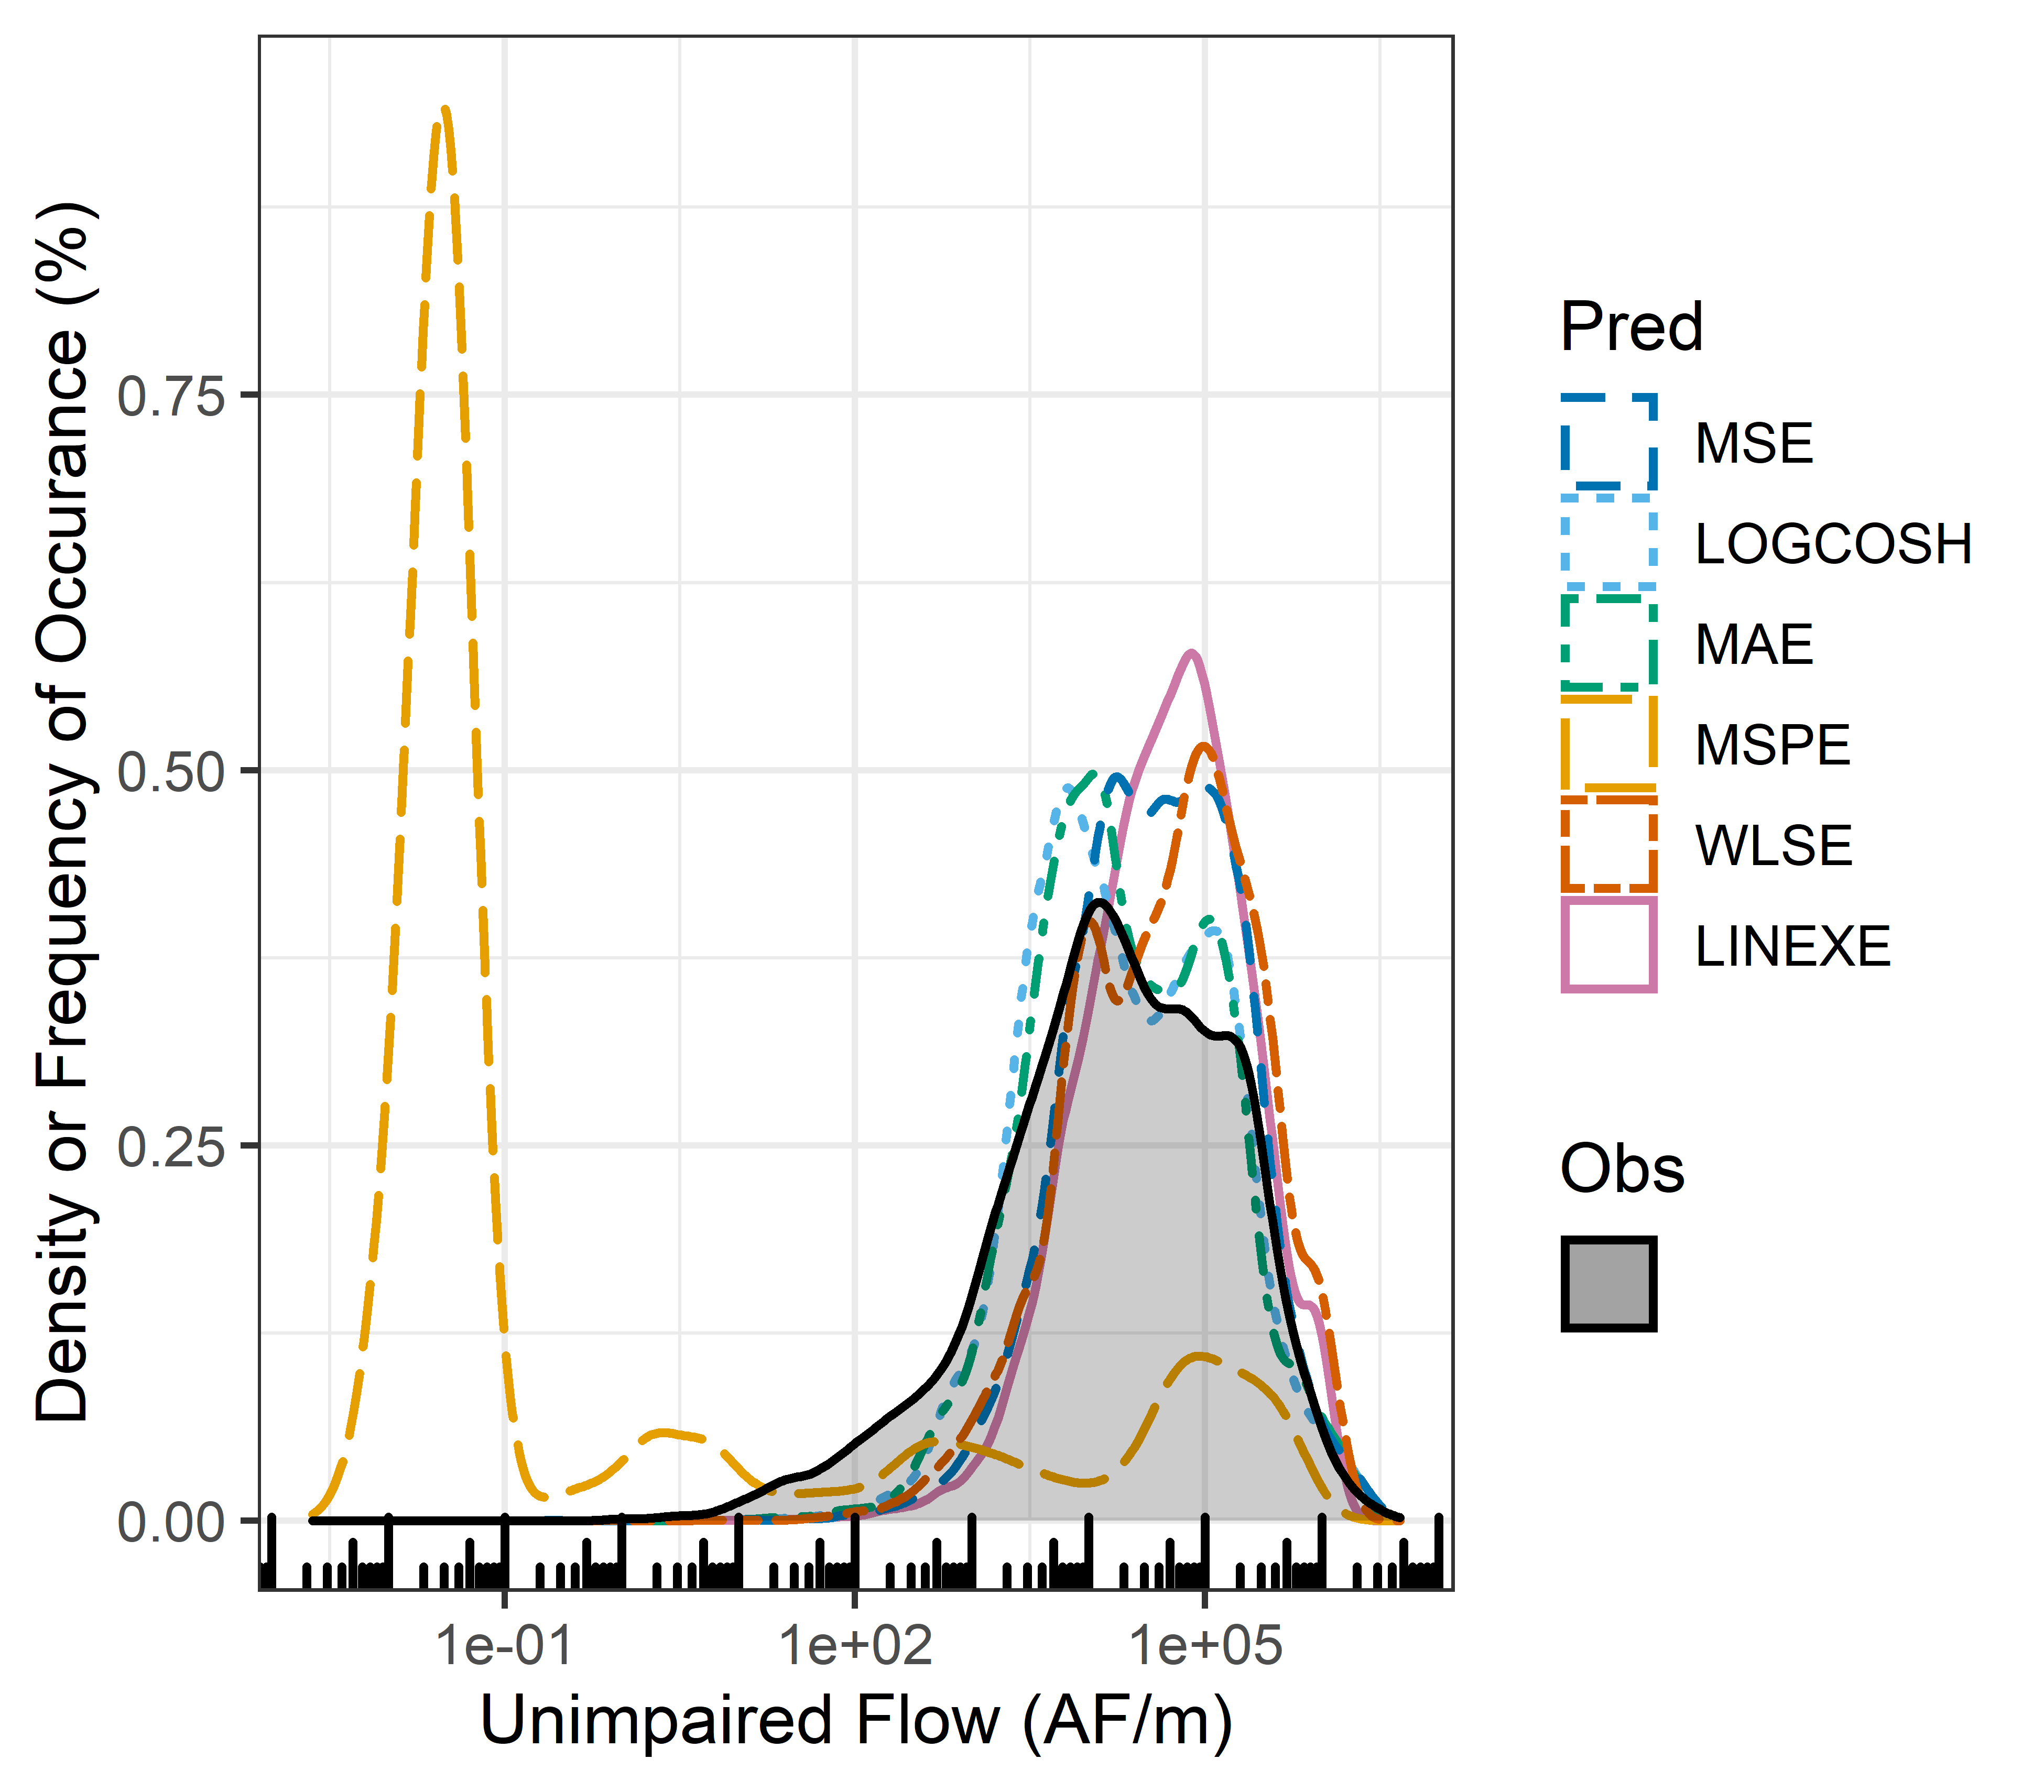
\includegraphics[width=\textwidth, trim={0 0 0 0}, clip=true]{plots/rplot34_density.png}
%  		\caption{Densities}
%  		\label{fig:density_obs}
%	\end{subfigure}% 
%	\begin{subfigure}{.5\textwidth}
%  		\centering
%  		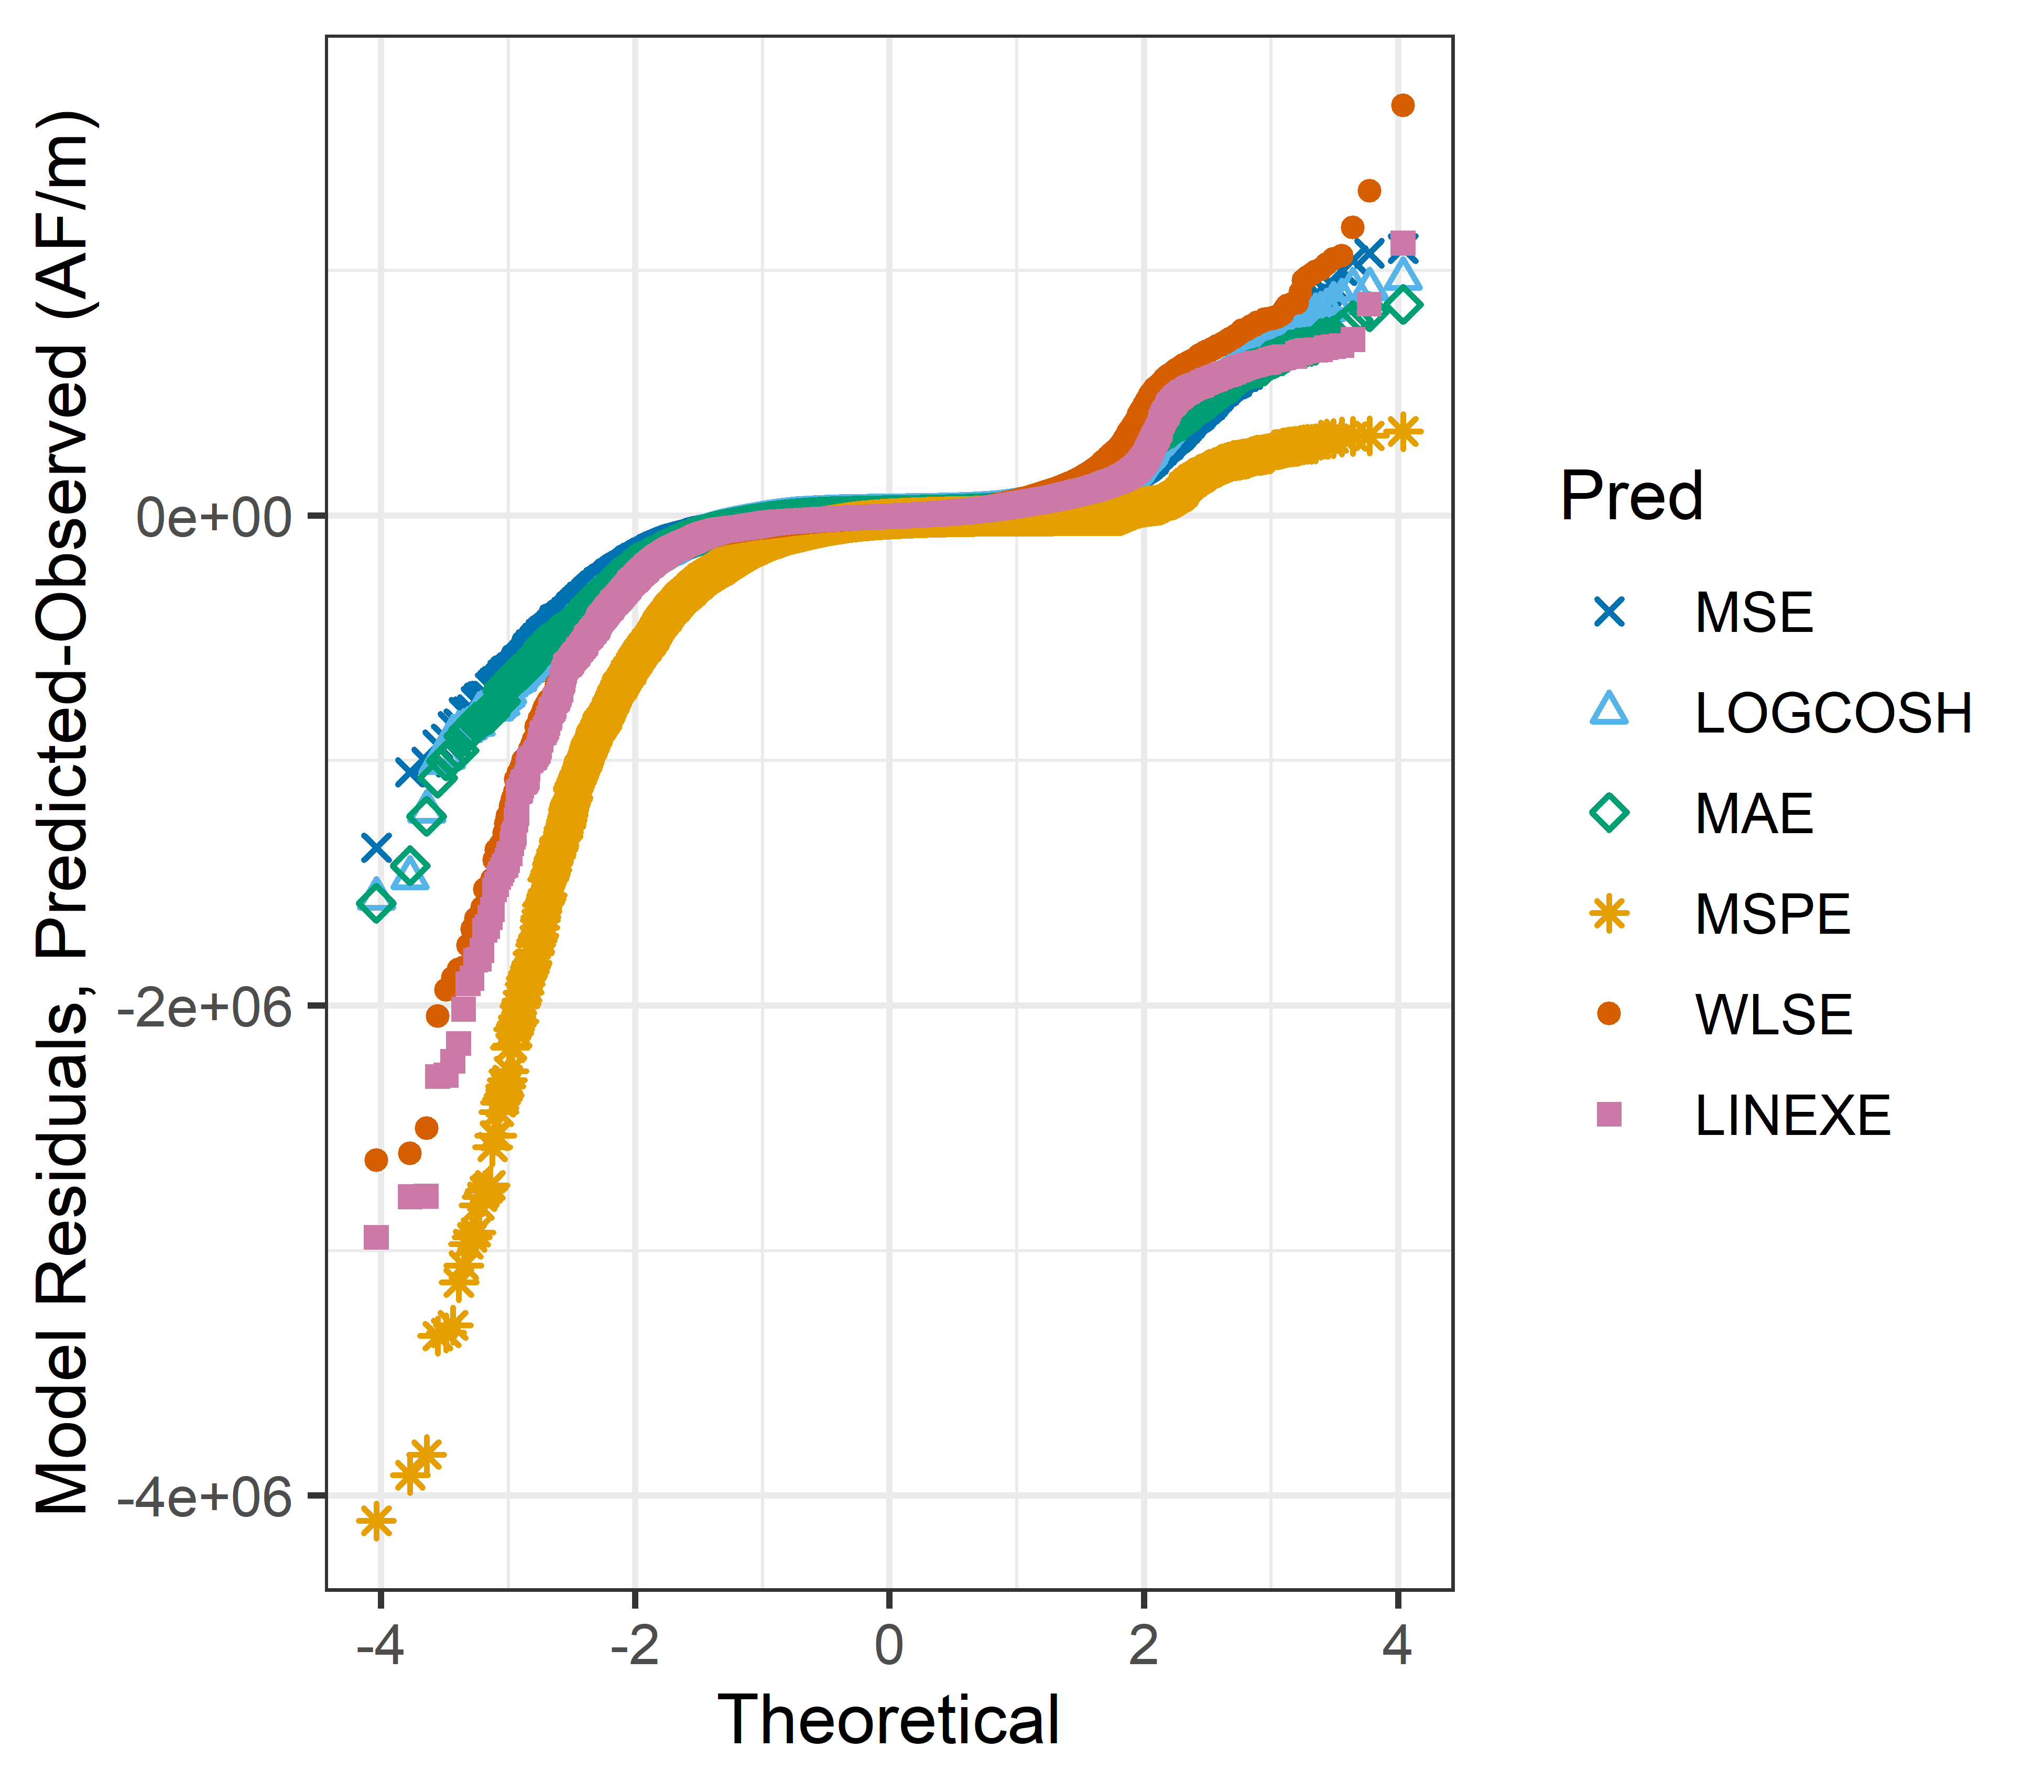
\includegraphics[width=\textwidth, trim={0 0 0 0}, clip=true]{plots/rplot34_qqplot_modelres.png}
%  		\caption{Q-Q plot}
%  		\label{fig:density_res}
%	\end{subfigure}
%	\caption[The probability densities of predictions, observations, and model residuals.]{ (b)}
%	\label{fig:density}
%\end{figure}

\begin{figure}
	\centering
	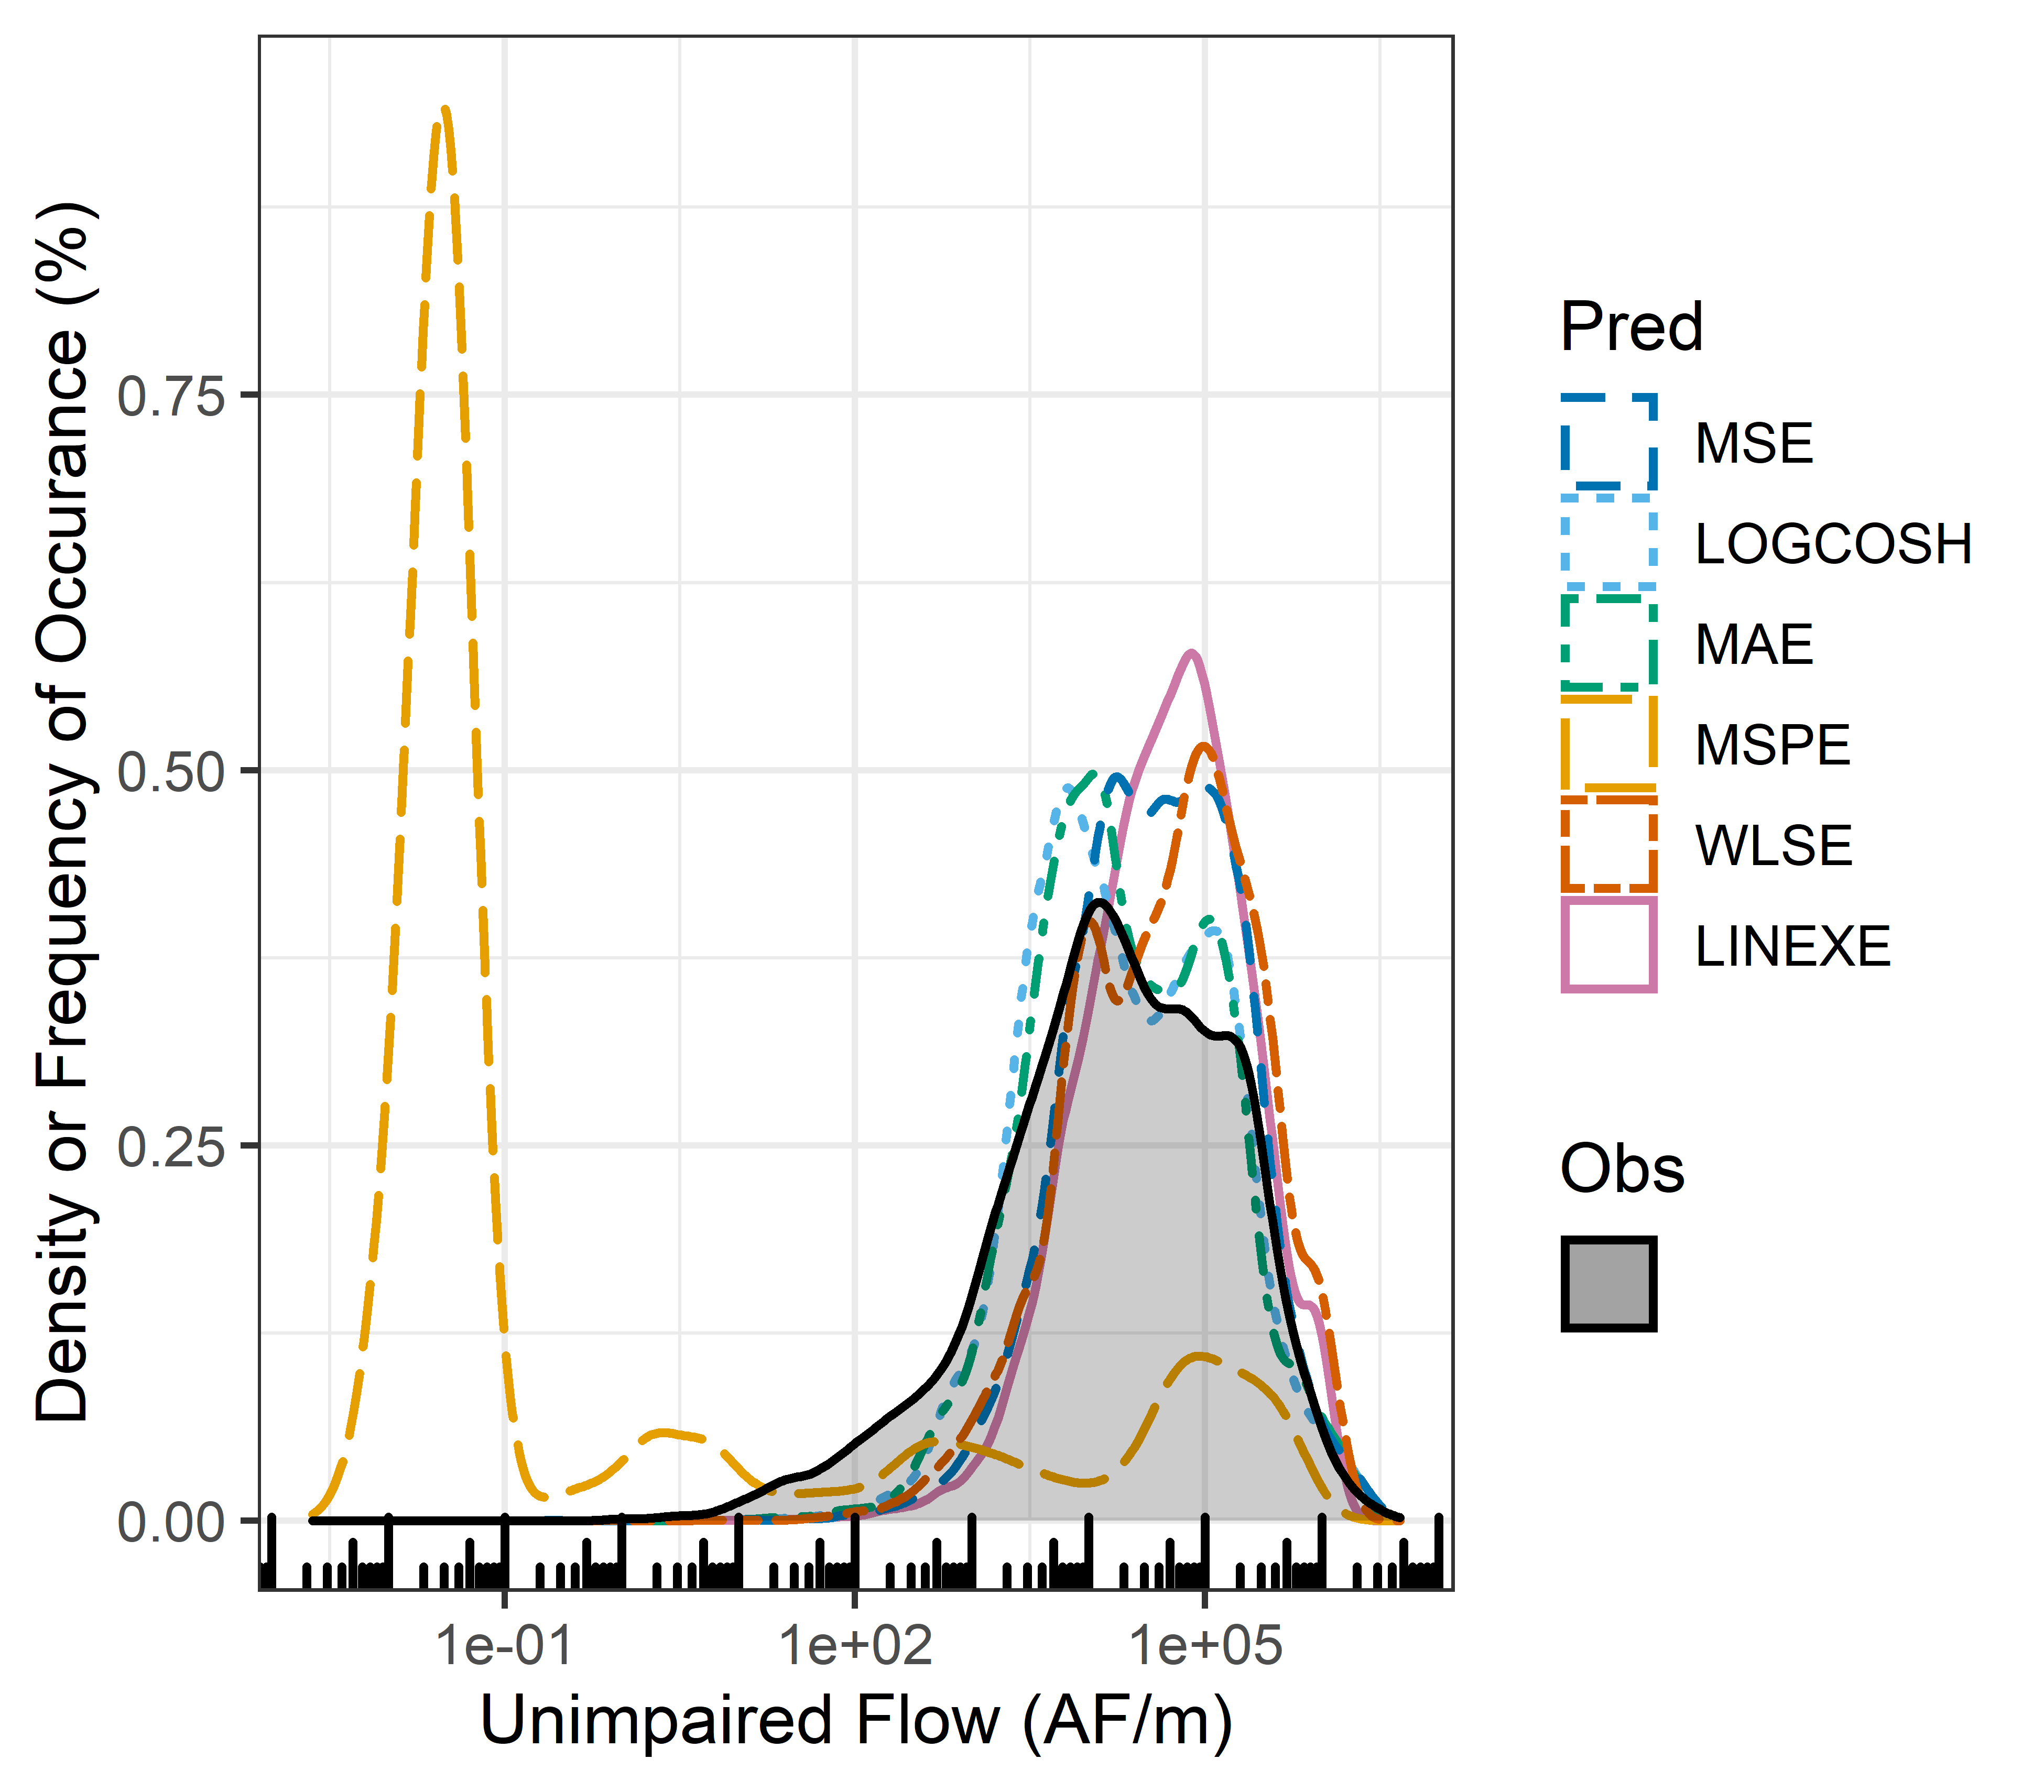
\includegraphics[width=0.5\textwidth, trim={0 0 0 0}, clip=true]{plots/rplot34_density.png}
	\caption[Probability densities of predictions and observations.]{Probability densities of predictions and observations. The MSPE is biased towards smaller predictions as there is a spike in the density (in orange) at the lower values compared to the observations (in black). The asymmetric losses predict larger floods more often (LINEXE > WLSE > MSE), which was their intended use. The MSE density (in dark blue) shows three peaks like the observations, except the floods get more pronounced. This shows the effects of having a squared error loss. The MAE and LOGCOSH perform very similarly predicting more droughts than floods. In contrast, the WLSE predicts more floods than droughts and the LINEXE predicts the most amount of floods.}
	\label{fig:densitych3}
\end{figure}

\begin{figure}[ht]
	\centering
	\begin{subfigure}{\textwidth}
  		\centering
 		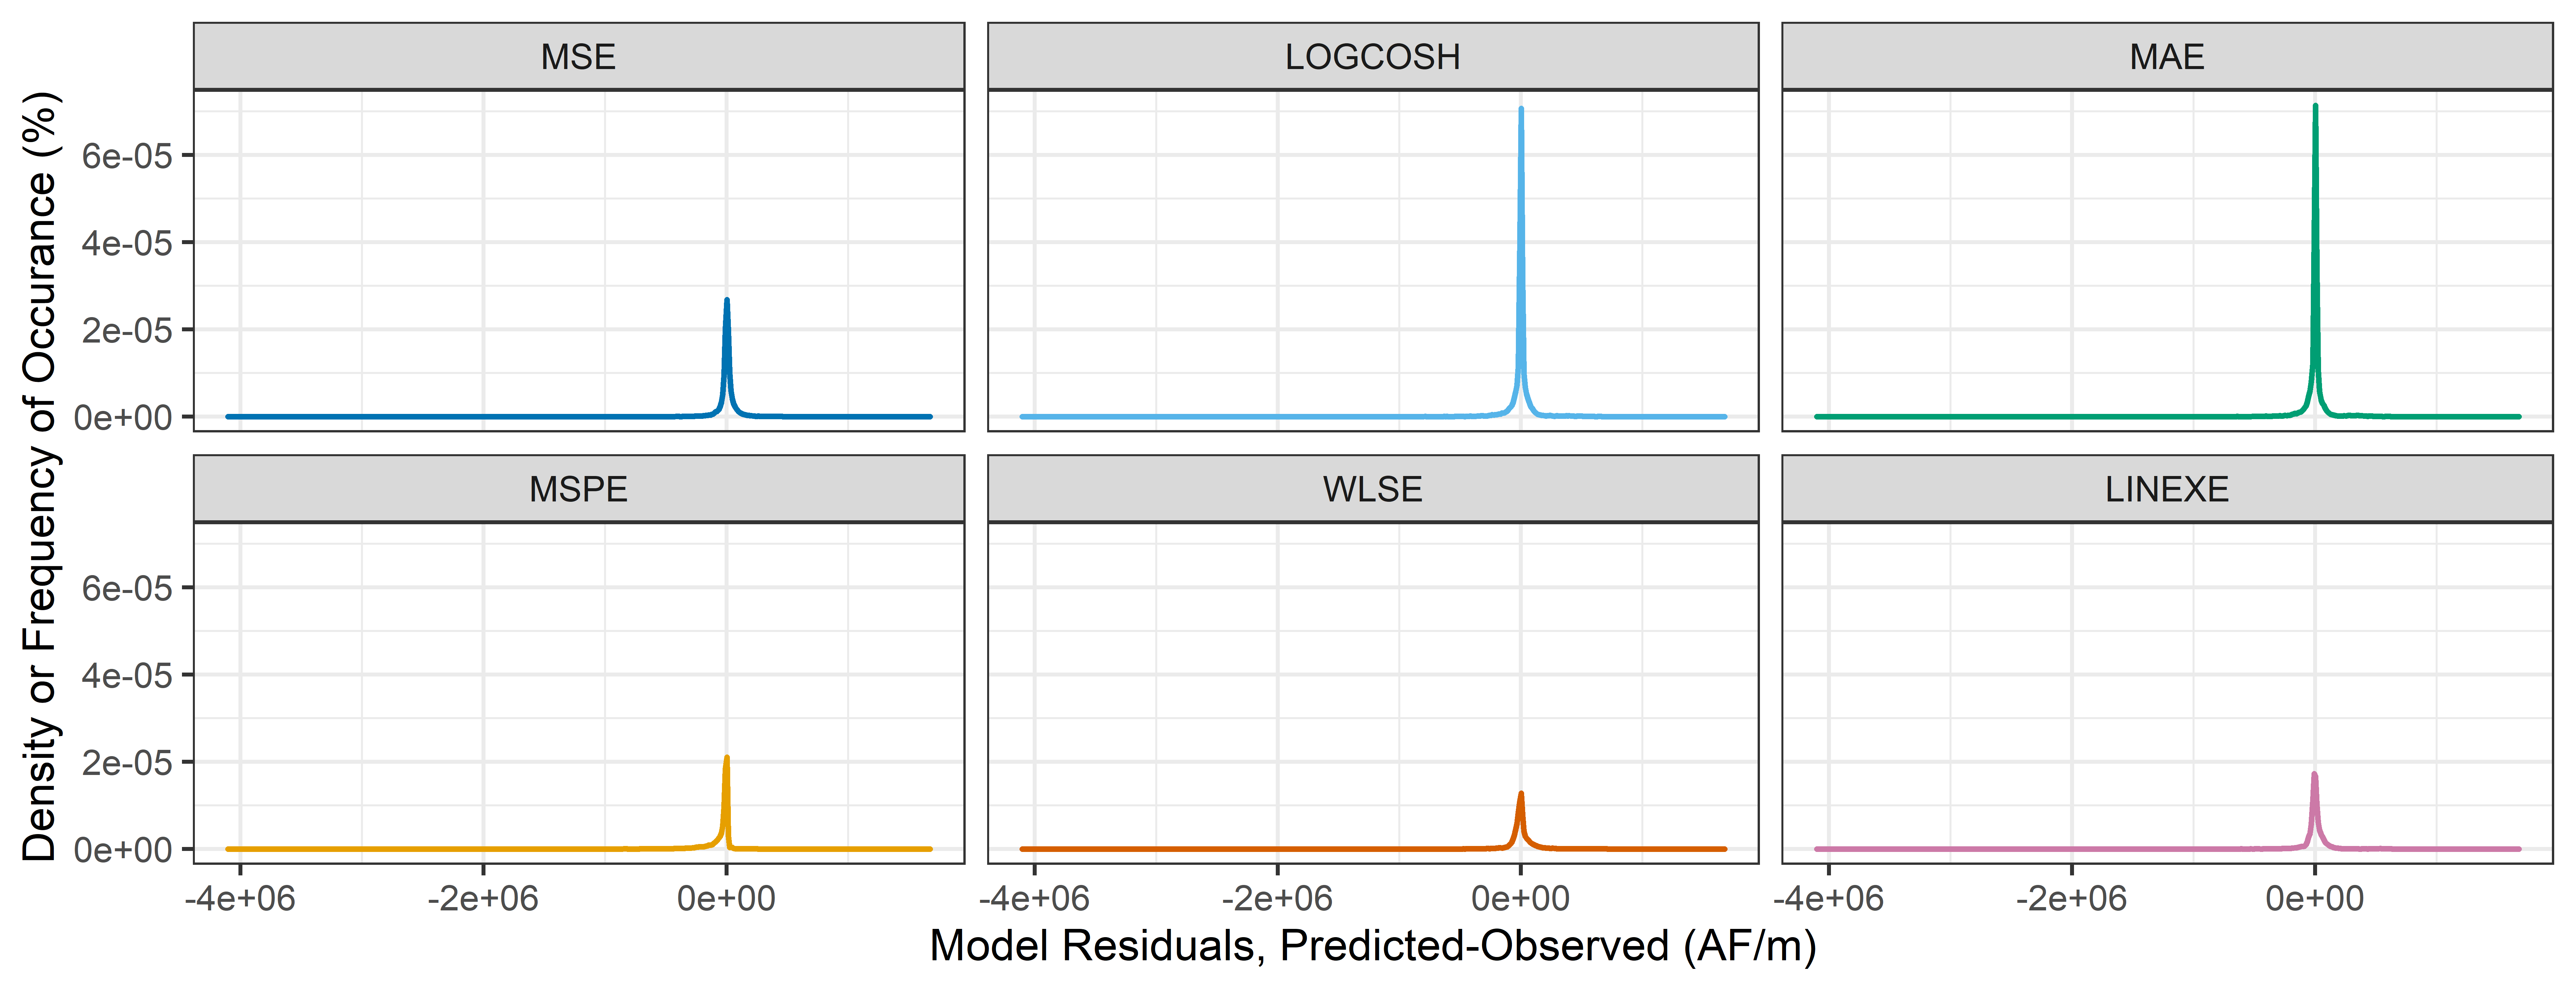
\includegraphics[width=\textwidth, trim={0 0 0 0}, clip=true]{plots/rplot34_density_res.png}
  		\caption{Residual error densities.}
  		\label{fig:density_obs}
	\end{subfigure}%
	\hfill
	\begin{subfigure}{.5\textwidth}
  		\centering
  		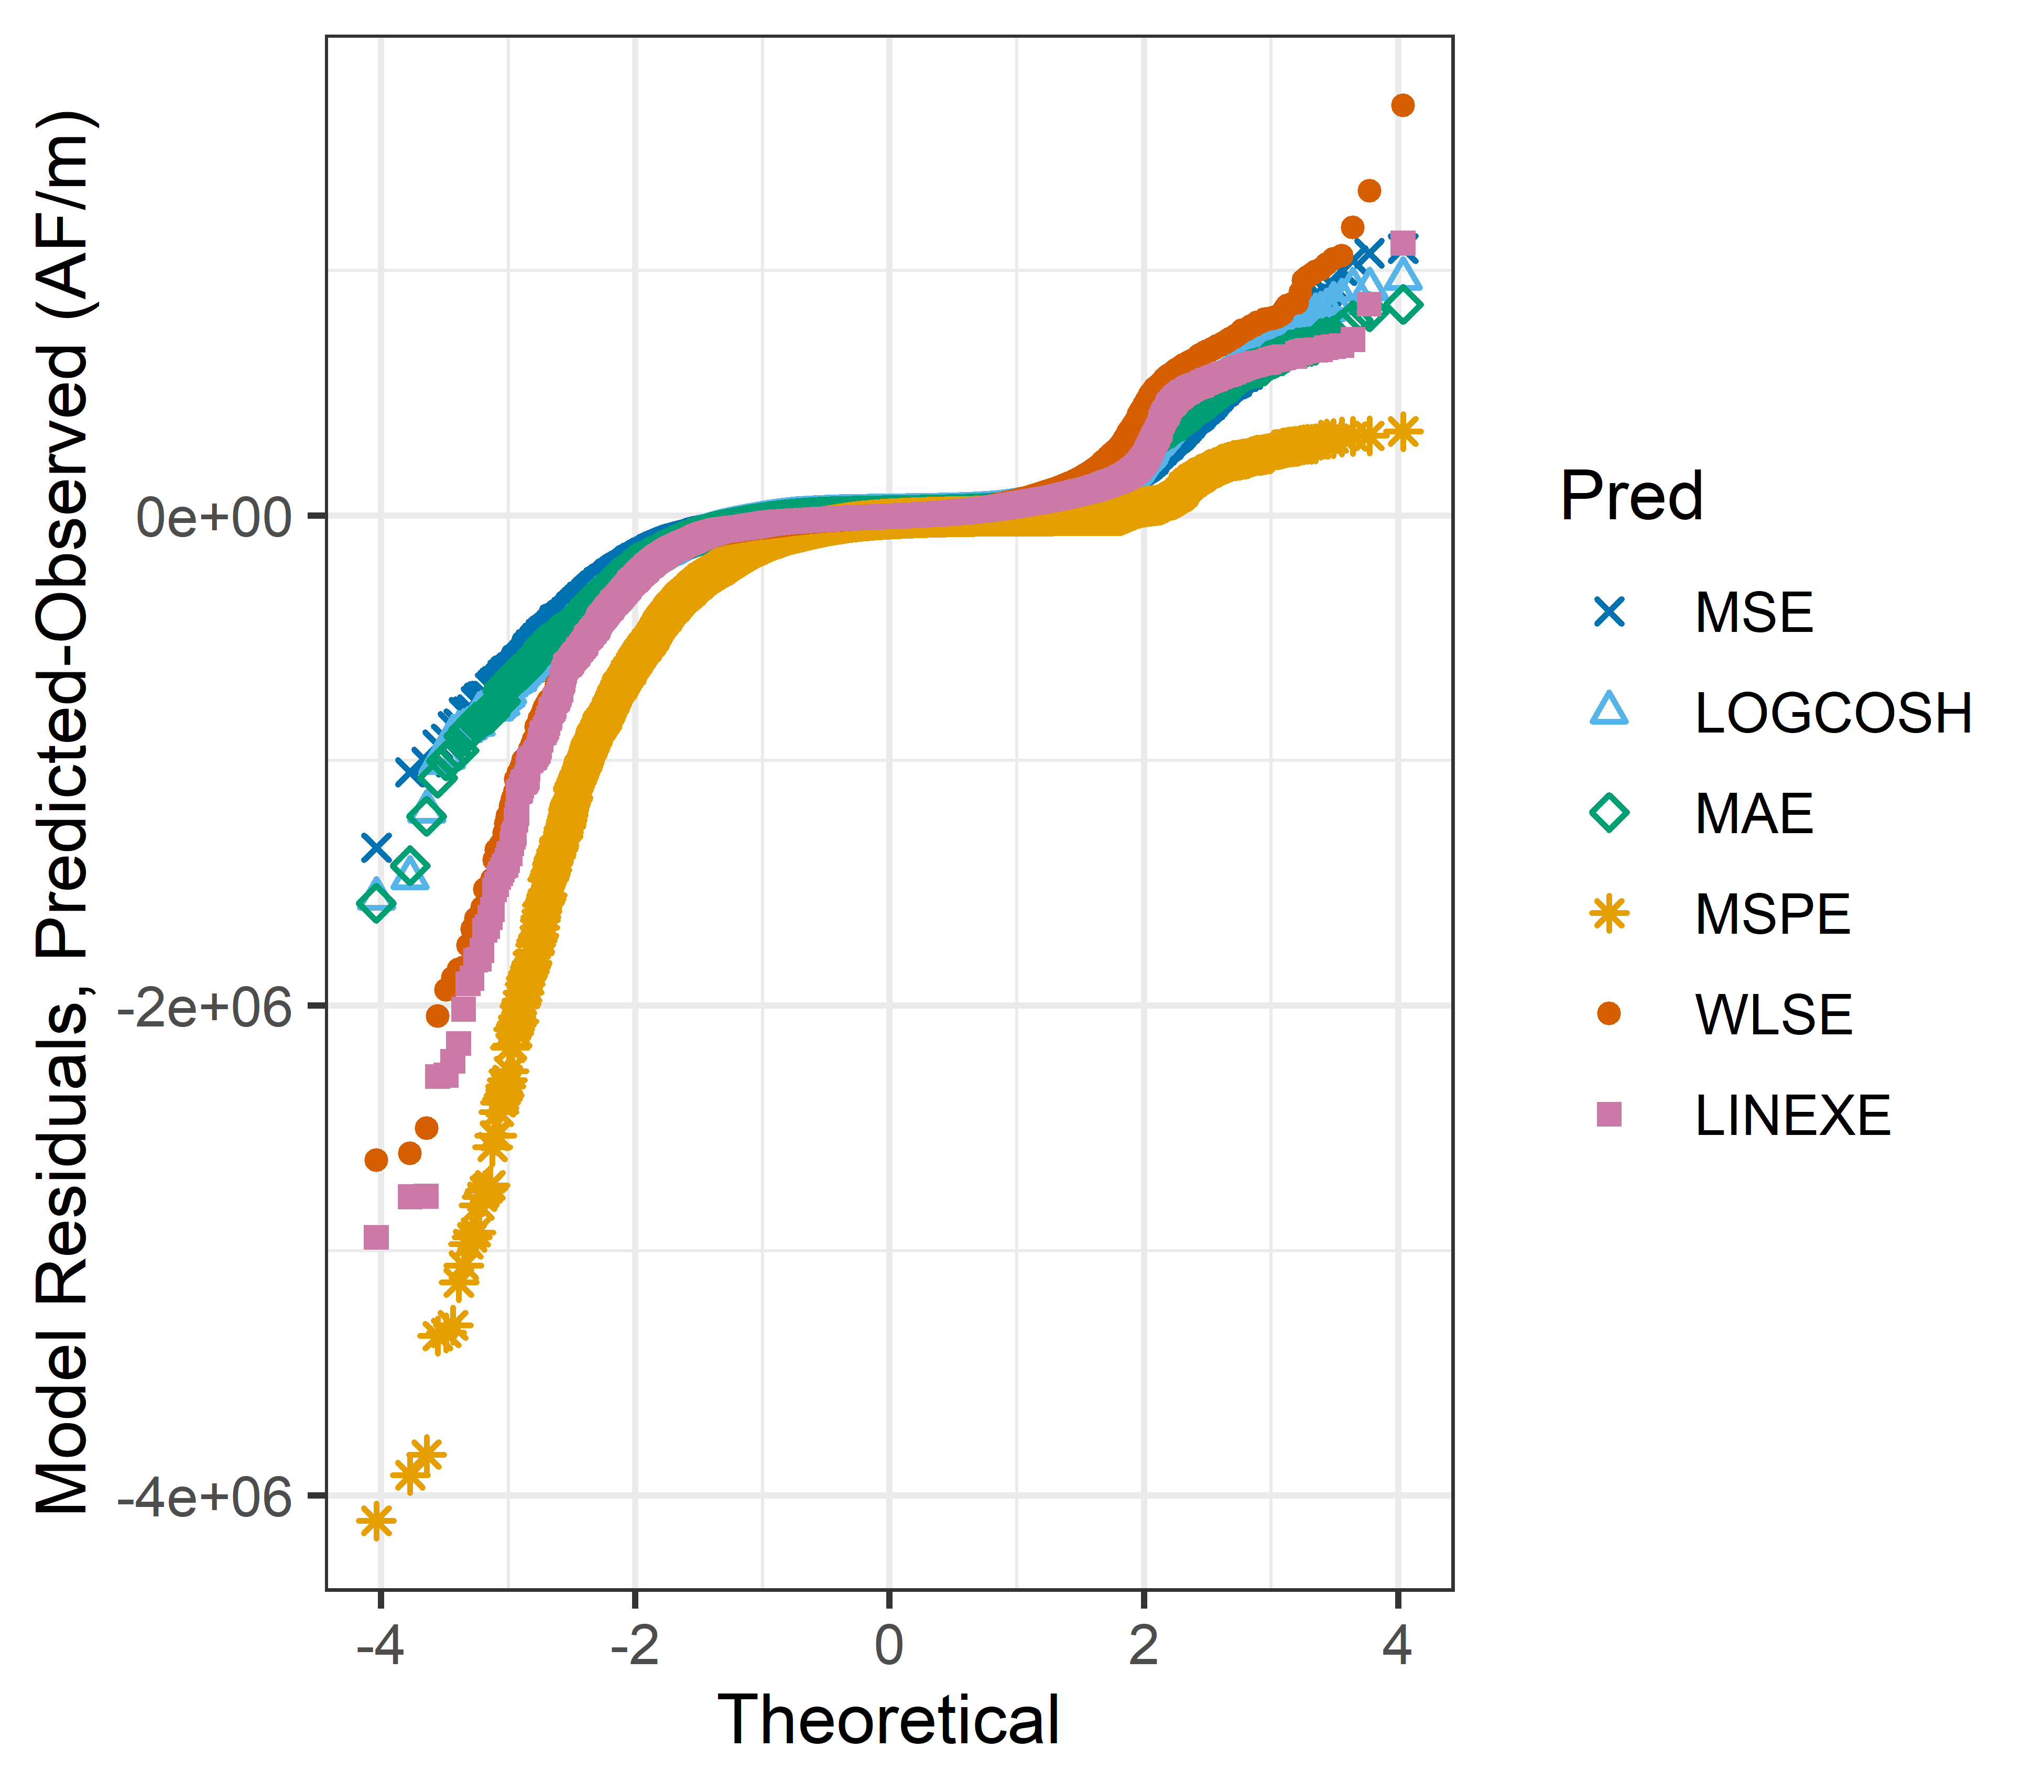
\includegraphics[width=\textwidth, trim={0 0 0 0}, clip=true]{plots/rplot34_qqplot_modelres.png}
  		\caption{Model residuals compared to a Normal distribution, Q-Q plot.}
  		\label{fig:density_res}
	\end{subfigure}
	\caption[Probability densities of model residual error.]{Probability densities of model residual error: (a) Model residuals are skewed left in all models, but is less extreme in WLSE and LINEXE; there is more of a tendency to underpredict floods in models, but less so in WLSE and LINEXE. (b) Model residuals do not have a normal distribution. The points fall along a line in the middle of the graph, but curve off in the extremities. This behavior implies that model residuals have more extreme values than would be expected if they truly came from a Normal distribution. WLSE shows the most extreme behavoir at higher levels (i.e., overpredicting floods).}
	\label{fig:reserrordens}
\end{figure}

Unsurprisingly, model residuals do not have a normal distribution (Figure \ref{fig:reserrordens}). The quantile-quantile plot is created by plotting two sets of quantiles against one another: one a sample (e.g., model residuals) and one the theoretical Normal distribution. Here, the points fall along a line in the middle of the graph, but curve off in the extremities. This behavior implies that model residuals have more extreme values than would be expected if they truly came from a Normal distribution.

In general, these densities show the amount of control the modeler has on the probability distribution of the predicted values when picking a loss function. This flexibility is especially useful in risk-based decision making where the modeling aim is to accurately predict the probability distribution particularly at its tails where high cost consequences may occur. A more direct way of approaching the problem is evaluating the goodness of the density estimate by calculating the generalization log-loss (or log-likelihood out-of-bag) and using conditional density estimation and ``probabilistic supervised learning'' methods. Models like Mixture Density Networks (MDN) not only predict the expected value of a target, but also the underlying probability distribution \cite{gressmann2018probabilistic, bishop1994mixture}.
%-----------------------------------------------
\subsection{Spatial Distribution of Error}
Figure \ref{fig:br2map} shows spatial performance for each loss function. Except for the MSPE which suffers from a major bias, other methods perform similarly. These methods favor the northern basins and watersheds lower in the network. The LINEXE and WLSE perform ``worse'' in headwater basins than the MSE because the asymmetry is pushing the model to underpredict at low flows. This effect is more pronounced in the WLSE than the LINEXE possibly due to the nuisance parameters. As explained before, the MSE, LOGCOSH and MAE perform similarly. 

\begin{figure}
	\centering
	\begin{frame}{}
        	\animategraphics[loop,controls]{1}{plots/ch3_gif_br2maps/rplot35_br2map_nn_}{1}{6}
	\end{frame}
	\caption[bR\textsuperscript{2} performance for different loss functions.]{bR\textsuperscript{2} performance for different loss functions. Except for the MSPE which suffers from a major bias, other methods perform similarly. These methods favor the northern basins and watersheds lower in the network.}
	\label{fig:br2map}
\end{figure}

%-----------------------------------------------------------------------------------------------------------------------------------------------------------------------------------------------------
\section{Conclusion} \label{ch4: conclusion}
This chapter followed a risk minimization framework in developing models with different loss functions. We \textit{are putting the horse before the cart}; the loss function is developed before performing the learning, not just as an evaluation step after. In squared error loss functions (i.e., MSE), the peaks or high leverage points get fitted at the expense of the low flows. 

The proposed WLSE and LINEXE asymmetric losses are able to force a fit to the tails of the distribution (the peaks and valleys of the hydrograph). These results are shown in the shape of the predicted time series compared to the observations. The LOGCOSH performs similarly to the MAE and MSE as is shown in the predicted vs. observed graphs and the bR\textsuperscript{2} measure. The MSPE is biased towards lower predictions and is not suited to problems where the data is skewed positive. 

In general, the differences show the amount of control the modeler has on the predictions and their probability distribution when picking a loss function. Many reasonable calibration loss functions exist, with somewhat different rationales that affect model estimates differently. The flexibility in picking a loss functions is especially useful in risk-based decision making where the modeling aim is to accurately predict the probability distribution particularly at its tails where high cost consequences may occur. Water managers can then uses this somewhat unbiased probability distribution in decision analysis. Asymmetric loss functions proved useful in this regard. 

%A dissertation chapter will include a comparison between the results of various loss functions applied. It will investigate the differences in the general shape of predictions obtained across the various loss functions, and discuss the effects of different weights in the asymmetric weighted MSE function.   

%Surprisingly, the models perform vastly different from one another depending on the objective function used, highlighting the importance of this much overlooked step. In summary, we define what loss means to a certain problem, we use that as the objective function in the machine learning algorithm, and then perform the minimization. 


% In statistical learning, with a pre-defined loss function we can estimate model parameters and then calculate the model measures-of-fit of interest. However, improving a model trained on a different loss function than that which is desired can be quite tricky. Since the machine learning algorithm requires a loss function to begin with, we can directly define the custom loss function as the measure-of-fit of interest before deploying the learning algorithm. This section performs statistical learning with different loss functions, and then examines the differences in predictions.
